\chapter{Implementation}
\textit{In this chapter, we address the implementation phase of the project. After establishing a detailed analysis and a clear design, the implementation represents the concrete culmination of our work, through the deployment of the various components of the project. We will detail here the main steps, the tools used, the challenges encountered, as well as the solutions provided.}
\pagebreak

\section{Work Technologies}
\textbf{Java:}
Java was the primary programming language for the development of this project. Java was chosen for its robustness, portability, and extensive ecosystem, which make it suitable for building scalable and maintainable applications. Its strong type system and mature libraries contributed to reliable code, while its widespread adoption ensured access to a large pool of resources and community support.
\begin{figure}[H]
\centering

\includegraphics[width=0.2\textwidth]{img/tech/java-logo.png}
\caption{Java logo}
\end{figure}

\textbf{Spring Boot:}
Spring Boot is a framework that simplifies the development of Java applications by providing auto-configuration and embedded servers. It enables rapid development of production-ready applications with minimal configuration, while offering comprehensive features for dependency injection, security, and data access.
\begin{figure}[H]
\centering

\includegraphics[width=0.3\textwidth]{img/tech/springboot-logo.png}
\caption{Spring Boot logo}
\end{figure}

\textbf{PostgreSQL:}
PostgreSQL is an advanced, open-source relational database management system known for its reliability, feature robustness, and performance. It was used as the primary database for this project, providing ACID compliance, advanced indexing, and support for complex queries and data types.
\begin{figure}[H]
\centering

\includegraphics[width=0.2\textwidth]{img/tech/postgres-logo.png}
\caption{PostgreSQL logo}
\end{figure}

\textbf{Redis:}
Redis is an in-memory data structure store used as a database, cache, and message broker. In this project, Redis was utilized for caching frequently accessed data and session management, significantly improving application performance and reducing database load.
\begin{figure}[H]
\centering

\includegraphics[width=0.2\textwidth]{img/tech/redis-logo.png}
\caption{Redis logo}
\end{figure}

\textbf{Docker:}
Docker is a platform for developing, shipping, and running applications in containers. It ensures that the application runs consistently across different environments, simplifying deployment and scaling while isolating dependencies.
\begin{figure}[H]
\centering

\includegraphics[width=0.3\textwidth]{img/tech/docker-logo.png}
\caption{Docker logo}
\end{figure}

\textbf{GitLab:}
GitLab is a software development platform that allows developers to collaborate, manage version control, and store their projects using Git, a distributed version control system.
\begin{figure}[H]
\centering

\includegraphics[width=0.3\textwidth]{img/logos/gitlab-logo.png}
\caption{GitLab logo}
\end{figure}

\textbf{IntelliJ IDEA:}
IntelliJ IDEA is a powerful integrated development environment (IDE) for Java development. It was used throughout the project for code development, debugging, and refactoring, providing intelligent code completion, advanced debugging tools, and seamless integration with build tools and version control systems.
\begin{figure}[H]
\centering

\includegraphics[width=0.3\textwidth]{img/tech/IntelliJ IDEA.png}
\caption{IntelliJ IDEA logo}
\end{figure}

\textbf{Excalidraw:}
Excalidraw is a virtual whiteboard tool for creating hand-drawn-like diagrams and sketches. It was used in this project for creating wireframes, system architecture diagrams, and visual representations of workflows, facilitating better communication and planning among team members.
\begin{figure}[H]
\centering

\includegraphics[width=0.3\textwidth]{img/logos/excalidraw-logo.png}
\caption{Excalidraw logo}
\end{figure}

\textbf{Apache Kafka:}
Apache Kafka is a distributed event streaming platform used for building real-time data pipelines and streaming applications. It allows for the efficient handling of large volumes of data in real-time, making it suitable for applications that require high throughput and low latency.
\begin{figure}[H]
\centering

\includegraphics[width=0.2\textwidth]{img/tech/kafka-logo.png}
\caption{Apache Kafka logo}
\end{figure}

\textbf{Apache Avro:}
Apache Avro is a data serialization framework that provides compact, fast, binary data format with rich data structures. It was used in this project for schema evolution and data serialization in Kafka messages, ensuring efficient data transmission and backward compatibility.
\begin{figure}[H]
\centering

\includegraphics[width=0.2\textwidth]{img/tech/apache-avro-logo.png}
\caption{Apache Avro logo}
\end{figure}

\textbf{Confluent Schema Registry:}
Confluent Schema Registry is a centralized repository for managing and validating schemas for topic message data. It works seamlessly with Apache Avro to provide schema evolution capabilities and ensures data compatibility across different versions of applications consuming Kafka topics.
\begin{figure}[H]
\centering

\includegraphics[width=0.3\textwidth]{img/tech/CFLT_BIG.png}
\caption{Confluent Schema Registry logo}
\end{figure}
\newpage

\section{Technical Results:}


\subsection{Performance tests and quality measures}
In this section, we will present the performance tests and quality measures applied to the codebase and stateless worker in runtime. These tests are essential to ensure that the application meets the expected performance standards and adheres to best practices in software development.
\subsection{Deployment}
In this section, we will present the technical results of the project, focusing on the deployment of the application and the tools used to ensure its quality. 
The deployment process is crucial as it allows us to make the application available for use and to ensure that it meets the expected standards of quality and security.


\begin{figure}
    \centering
    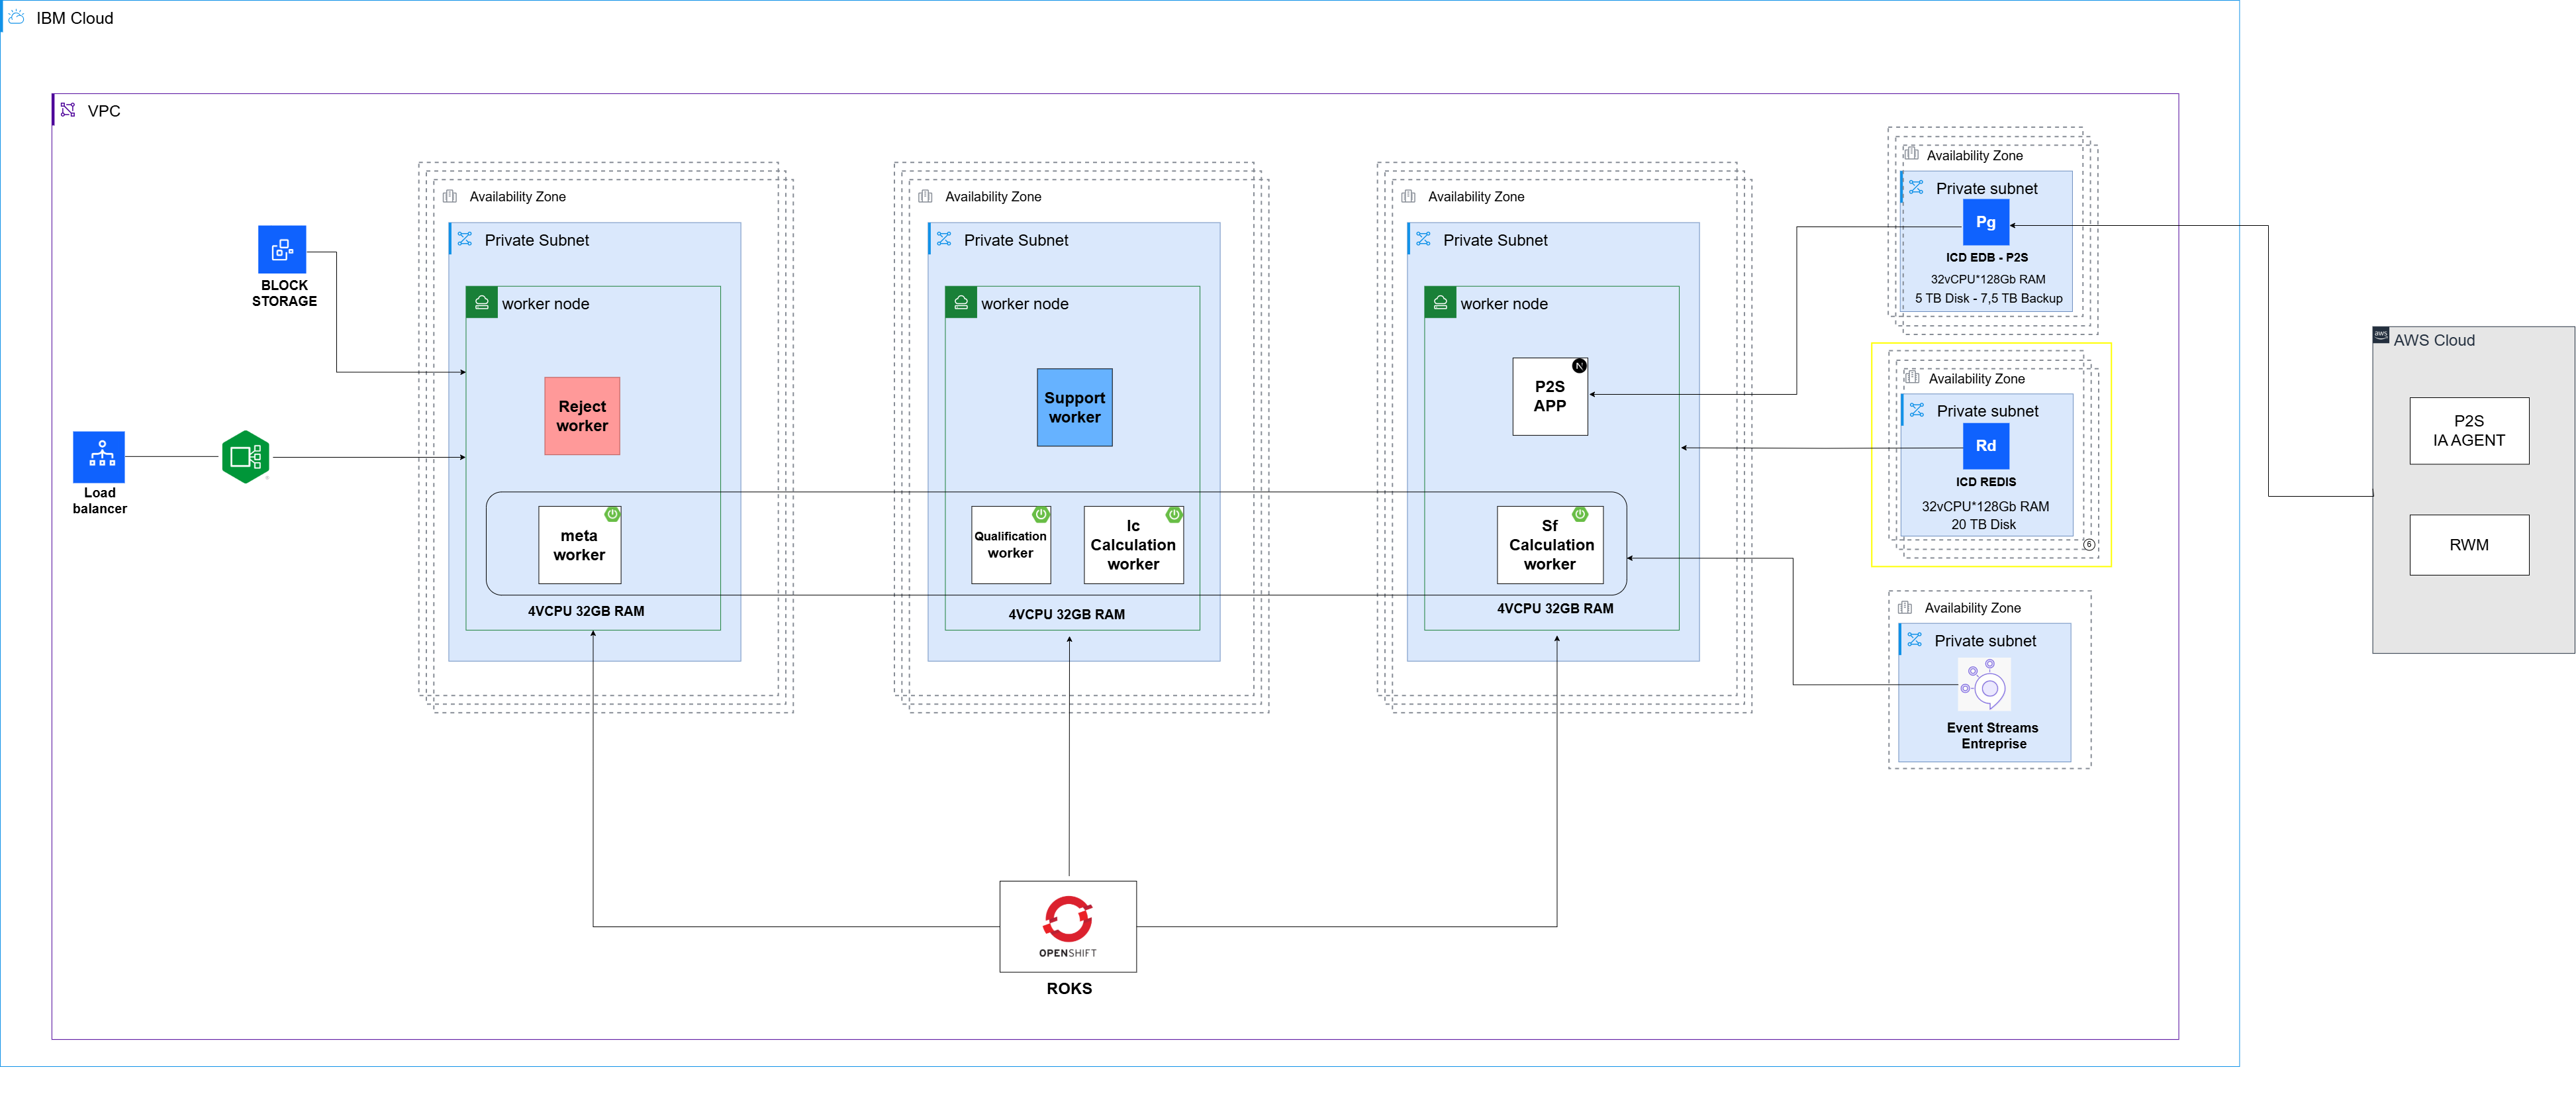
\includegraphics[width=1\textwidth]{img/arch/p2s-workers-deployment.drawio.png}
    \caption{Deployment Architecture}
    \label{fig:deployment}
\end{figure}
  
This architectural deployment demonstrates a distributed microservices approach optimized for high-availability transaction processing within IBM Cloud's multi-zone infrastructure. The system leverages  availability zones to ensure fault tolerance and geographic distribution, the compute engines deployed as instances in all availability zones as independent worker nodes provisioned with sufficient resources  to handle intensive financial calculations. 
The Meta Worker serves as the intelligent transaction dispatcher, while the second zone hosts the Context Qualification and Interchange Calculation engines responsible for transaction evaluation and fee computation. The third zone contains the Scheme Fees Calculation engine alongside the primary P2S application components.
This zonal distribution strategy ensures that critical processing components remain operational even during zone-level failures, while the stateless nature of each worker enables horizontal scaling based on transaction volume demands. The integration with ROKS (Red Hat OpenShift) provides container orchestration capabilities, while the Event Streams Enterprise implementation facilitates reliable Kafka-based messaging between components. The hybrid cloud approach, incorporating AWS services for extended P2S functionality, demonstrates the system's ability to leverage best-of-breed services across multiple cloud providers while maintaining centralized control within the IBM Cloud VPC infrastructure.


% \section{Quality Measures}

% This section provides an overview of the quality measures used to evaluate the codebase, focusing on the following tools: \texttt{Flake8}\cite{flake8}, \texttt{Radon}\cite{radon}, and \texttt{Bandit}\cite{bandit}. The results obtained from these tools are presented, followed by an analysis.

% \subsection{Flake8 Overview}
% Flake8 is a Python tool for enforcing coding standards. It checks the code for compliance with the PEP 8 style guide and also looks for potential errors and issues that could affect code quality. Flake8 can detect:
% \begin{itemize}
%     \item Syntax errors
%     \item Undefined names
%     \item Coding style violations
%     \item Potentially problematic constructs
% \end{itemize}
% It combines the functionality of several Python linting tools: \texttt{pyflakes}, \texttt{pycodestyle}, and \texttt{mccabe}. The tool helps maintain a consistent coding style and catch common mistakes early in the development process.

% \subsection{Radon Overview}
% Radon is a Python tool used for computing various software metrics that help assess code quality. The metrics provided by Radon focus on complexity, maintainability, and overall code health. Key metrics calculated by Radon include:

% \subsubsection{Cyclomatic Complexity (CC)}
% Cyclomatic Complexity measures the number of linearly independent paths through the code. It is calculated by analyzing the Abstract Syntax Tree (AST) of the code and counting the number of decision points (such as `if`, `for`, `while`, `except`, etc.). A higher value of CC indicates more complex code, which may require more effort to test and maintain.

% \subsubsection{Maintainability Index (MI)}
% The Maintainability Index is a composite metric that combines several factors, including Cyclomatic Complexity, Halstead Volume, and Source Lines of Code (SLOC). It provides an estimate of how easy it is to maintain a codebase. The formula used by Radon is:

% \[
% MI = \max\left[0, 100 \times \left(171 - 5.2 \ln V - 0.23 G - 16.2 \ln L + 50 \sin\left(\sqrt{2.4 C}\right)\right) / 171 \right]
% \]

% Where:
% \begin{itemize}
%     \item \(V\) = Halstead Volume,
%     \item \(G\) = Cyclomatic Complexity,
%     \item \(L\) = Source Lines of Code (SLOC),
%     \item \(C\) = percentage of comment lines (converted to radians).
% \end{itemize}

% A higher MI value generally indicates more maintainable code.

% \subsubsection{Raw Metrics}
% Raw metrics provided by Radon include:
% \begin{itemize}
%     \item \textbf{LOC (Lines of Code)}: Total number of lines, including blank lines and comments.
%     \item \textbf{LLOC (Logical Lines of Code)}: The number of lines that contain a single statement.
%     \item \textbf{SLOC (Source Lines of Code)}: The number of lines of actual code, excluding comments and blank lines.
%     \item \textbf{Comments}: The number of comment lines.
%     \item \textbf{Multi}: The number of lines that represent multi-line strings.
%     \item \textbf{Blanks}: The number of blank lines.
% \end{itemize}

% The equation \( \text{SLOC} + \text{Multi} + \text{Single comments} + \text{Blank} = \text{LOC} \) should always hold. Additionally, comment stats are calculated:

% \[
% C \% L = \frac{\text{Number of comment lines}}{\text{LOC}} \times 100
% \]
% \[
% C \% S = \frac{\text{Number of comment lines}}{\text{SLOC}} \times 100
% \]
% \[
% C + M \% L = \frac{\text{Number of comment and multiline strings lines}}{\text{LOC}} \times 100
% \]

% \subsubsection{Halstead Metrics}
% Halstead's goal was to identify measurable properties of software and the relationships between them. These numbers are statically computed from the source code:

% \begin{itemize}
%     \item \( \eta_1 \) = the number of distinct operators
%     \item \( \eta_2 \) = the number of distinct operands
%     \item \( N_1 \) = the total number of operators
%     \item \( N_2 \) = the total number of operands
% \end{itemize}

% From these numbers, several measures can be calculated:

% \begin{itemize}
%     \item \textbf{Program Vocabulary:} 
%     \[
%     \eta = \eta_1 + \eta_2
%     \]
    
%     \item \textbf{Program Length:} 
%     \[
%     N = N_1 + N_2
%     \]
    
%     \item \textbf{Calculated Program Length:} 
%     \[
%     \hat{N} = \eta_1 \log_2 \eta_1 + \eta_2 \log_2 \eta_2
%     \]
    
%     \item \textbf{Volume:} 
%     \[
%     V = N \log_2 \eta
%     \]
    
%     \item \textbf{Difficulty:} 
%     \[
%     D = \frac{\eta_1}{2} \cdot \frac{N_2}{\eta_2}
%     \]
    
%     \item \textbf{Effort:} 
%     \[
%     E = D \cdot V
%     \]
    
%     \item \textbf{Time Required to Program:} 
%     \[
%     T = \frac{E}{18} seconds
%     \]
    
%     \item \textbf{Number of Delivered Bugs:} 
%     \[
%     B = \frac{V}{3000}
%     \]
% \end{itemize}


% \subsection{Bandit Overview}
% Bandit is a tool designed to find security issues in Python code. It performs static analysis to identify potential vulnerabilities, such as:
% \begin{itemize}
%     \item SQL injection risks
%     \item Use of weak cryptographic algorithms
%     \item Insecure file handling
%     \item Insecure deserialization
%     \item Hardcoded passwords or tokens
% \end{itemize}
% Bandit provides an automated way to identify security risks, which is especially valuable in ensuring that the code does not have common vulnerabilities.

% \subsection{Results}
% The following plot presents the results obtained from running Flake8, Radon, and Bandit on the codebase. These results offer a quantitative assessment of the code quality and security.

% % Include the plot here
% \begin{table}[ht!]
%     \centering
%     \begin{tabular}{|l|l|}
%     \hline
%     \textbf{Metric}               & \textbf{Value}                        \\ \hline
%     Halstead's \(\eta_1\) (distinct operators)   & 12                                      \\ \hline
%     Halstead's \(\eta_2\) (distinct operands)    & 66                                      \\ \hline
%     Total number of operators \(N_1\)             & 40                                      \\ \hline
%     Total number of operands \(N_2\)              & 80                                      \\ \hline
%     Program vocabulary \(\eta\) & 78                                      \\ \hline
%     Program length \(N\)              & 120                                     \\ \hline
%     Calculated program length \(\hat{N}\) & 441.95                                 \\ \hline
%     Volume \(V \)               & 754.25                                  \\ \hline
%     Difficulty \(D \)   & 7.27                                      \\ \hline
%     Effort \(E\)                      & 5485.44                                 \\ \hline
%     Time required to program \(T\) & 304.75                                  \\ \hline
%     Number of delivered bugs \(B \) & 0.2514                                 \\ \hline
%     \end{tabular}
%     \caption{Halstead Metrics Results}
%     \end{table}
    

% \subsection{Analysis}
% The results from Flake8, Radon, and Bandit provide a comprehensive view of the code's quality and security. Based on the plot, the following observations can be made:

% \begin{itemize}
%     \item \textbf{Flake8 Results}: The Flake8 results indicate the adherence of the code to the PEP 8 guidelines, with a few minor coding style violations. These violations should be addressed to improve the consistency and readability of the code.
%     \item \textbf{Radon Results}: The Radon metrics reveal that the code has a moderate level of Cyclomatic Complexity, indicating that there may be some areas that could be refactored to reduce complexity. The Maintainability Index suggests that the code is maintainable but could benefit from simplification in certain parts.
%     \item \textbf{Bandit Results}: The Bandit results show that the code is free of critical security vulnerabilities, but some medium severity issues may require attention.
% \end{itemize}

% In conclusion, while the codebase appears to be in good shape, addressing the identified issues will improve both its maintainability and security. Refactoring complex sections of code, improving coding style, and addressing minor security concerns will help enhance the overall quality of the project.


\section{Conclusion}
With this final step, we have completed the implementation of the project by applying the analytical and conceptual studies presented in the second chapter. We have presented the tools used for its development as well as the various interfaces that were created.
\pagebreak
